% !TEX root = ../notes_unsupervisedlearning.tex
% Chapter 13: World Models
%%%%%%%%%%%%%%%%%%%%%%%%%%%%%%%%%%%%%%%%%%%%%%%%%%%%%%%%%%%%%%%%%%%%%%

\chapter{World Models}\index{World Models}\index{Dreamer}\index{model-based RL}
\printchapterversion{13_world_models}
\newthought{Simulate, imagine, then act.}

%═══════════════════════════════════════════════════════════════════════
% BLOCK 1: INTRODUCTION
%═══════════════════════════════════════════════════════════════════════

\section{The Why}\index{world model}\index{model-based RL}\index{sample efficiency}

\marginnote{\newthought{World model.}\index{world model} A learned, generative model of an environment's dynamics
that takes a state and an action and returns a predicted next state and reward.
The agent can then roll out trajectories in this model rather than in the real environment,
and a policy trained on those imagined rollouts is said to plan in imagination.}

\newthought{In the previous chapter} we asked humans to do the heavy lifting,
querying labels, correcting the agent online, and demonstrating the task by hand.
Model-free reinforcement learning and imitation share a common cost,
both need an enormous number of rollouts in the real environment to converge.
This chapter learns a model of the environment instead,
so that planning, exploration, and policy improvement can happen in imagination
at a fraction of the data and risk.

\marginnote{\newthought{Real versus imagined.}\index{simulation}
One hour of robot interaction in the physical world can cost more than a week
of GPU time spent rolling out trajectories in a learned simulator.
The asymmetry between real interaction and imagined interaction is the structural fact
that motivates this chapter.}

\marginnote{\newthought{Sample efficiency.}\index{sample efficiency} The number of environment interactions
a method needs to reach a given level of performance. Model-free RL is famously sample-inefficient,
and model-based methods amortise expensive real interaction by training the policy on cheap imagined rollouts
inside the learned world model.}

\newthought{Real interaction is the bottleneck.}
Each environment step costs wall-clock time, hardware wear, and exposure to safety risk.
A simulator narrows the gap but introduces sim-to-real mismatch,
and the agent that crosses that gap still pays for every real rollout it then needs to fine-tune.
Sample efficiency is not a luxury, it is what decides whether a method ever leaves the lab.

\newthought{Dynamics models and Dyna-style planning.}\index{model-based RL}
Learn a transition function $f_\theta(s, a) \approx (s', r)$ from collected experience,
then use it to generate synthetic transitions that augment the real ones during policy updates.
The agent improves its policy from far fewer real interactions
because most of the gradient signal comes from the model.

\newthought{Latent world models.}\index{Ha-Schmidhuber world model}
Ha and Schmidhuber compress observations into a low-dimensional latent
and learn dynamics in that latent space~\cite{Ha2018WorldModels}.
A vision module encodes pixels, a recurrent memory module predicts future latents,
and a small controller is trained entirely on the imagined rollouts.

\marginnote{\newthought{Atari from imagination.}\index{Dreamer}\index{Atari}
Dreamer learned to play a wide range of Atari games from latent rollouts alone~\cite{Hafner2020Dreamer}.
The actor-critic never saw a real frame at training time, only the world model's predicted ones,
yet the policy transferred to the real environment without further interaction.
The world-model imagination served the same role for the policy gradient
that the replay buffer played in DQN, but with synthetic data instead of stored transitions.}

\newthought{Dreamer and latent imagination.}\index{Dreamer}
Dreamer learns a recurrent state-space model jointly with a reward predictor
and trains an actor-critic on trajectories rolled out in latent space~\cite{Hafner2020Dreamer}.
Backpropagating value gradients through the imagined dynamics
turns the world model into a differentiable simulator that the policy can be optimised against.

\marginnote{\newthought{Compounding error.}\index{compounding error} The accumulation of per-step prediction
errors as a learned model is rolled out over a horizon. Errors compound roughly linearly in the horizon length,
which is why short horizons, ensembles, frequent re-planning, and physics priors all show up as
mitigations later in the chapter.}

\newthought{Curiosity-driven exploration.}\index{curiosity}\index{ICM}
When extrinsic reward is sparse, an intrinsic bonus for visiting states the model fails to predict
gives the agent a reason to explore.
The Intrinsic Curiosity Module measures novelty as forward-model prediction error~\cite{Pathak2017Curiosity},
turning the world model itself into a source of exploration signal.

\marginnote{\newthought{Sim-to-real gap.}\index{sim-to-real gap} The difference between a simulator's
dynamics and the real environment's, which determines how much real-world fine-tuning a sim-trained policy
needs after transfer. Domain randomisation and physics priors are two strategies for narrowing the gap;
the world model is a third, since the simulator and the policy are now fitted jointly.}

\newthought{Random Network Distillation.}\index{RND}
Prediction-error curiosity has a known failure mode,
the agent fixates on stochastic noise it can never learn to predict.
Random Network Distillation replaces the forward model with a frozen random target
and rewards the inability of a learned network to match it~\cite{Burda2019RND},
yielding a novelty signal that ignores irreducible randomness in the observation.

\newthought{Physics priors and inductive biases.}\index{physics-informed}
Pure data-driven dynamics drift over long horizons because nothing penalises non-physical predictions.
Physics-informed neural networks add a residual loss that anchors the model to known equations of motion~\cite{Raissi2019PINN},
and Lagrangian or Hamiltonian parameterisations build conservation laws into the architecture itself
so that imagined rollouts respect the structure of the real world.

\newthought{In order to move from trial and error in the real world to planning in imagination}
we have good reason to find ways to,
\begin{itemize}
    \item learn dynamics models from collected experience,
    so that policy improvement is paid for in GPU time rather than hardware wear.
    \item compress observations into a latent space and predict in that space,
    so that the world model can be trained jointly with a reward predictor and rolled out efficiently.
    \item train policies on rollouts inside the learned model,
    treating the world model as a differentiable simulator the agent can be optimised against.
    \item drive exploration with intrinsic signals derived from the model,
    so that sparse extrinsic reward does not stall learning.
    \item encode physical structure as prior or as architecture,
    so that errors in the imagined dynamics do not compound unchecked across long horizons.
\end{itemize}

\newthought{The fundamental question} this chapter answers is whether an agent can learn enough
about its environment to do most of its thinking in its own head,
trading expensive real interaction for cheap imagined rollouts
without losing touch with the world it eventually has to act in.

\newpage

\iffalse
\subsection{Hands On Experience}

\begin{marginfigure}
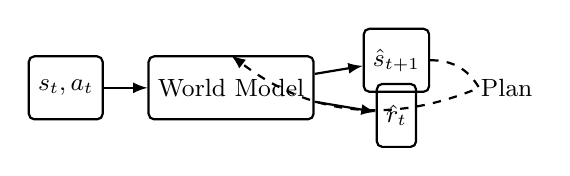
\begin{tikzpicture}[scale=0.7,
    every node/.style={font=\small},
    box/.style={draw, rectangle, rounded corners=2pt, thick, minimum height=0.8cm}]
    \node[box, minimum width=2cm] (wm) at (0,0) {World Model};
    \node[box] (s) at (-3,0) {$s_t, a_t$};
    \node[box] (sp) at (3,0.5) {$\hat{s}_{t+1}$};
    \node[box] (r) at (3,-0.5) {$\hat{r}_t$};

    \draw[-latex, thick] (s) -- (wm);
    \draw[-latex, thick] (wm) -- (sp);
    \draw[-latex, thick] (wm) -- (r);

    \draw[-latex, thick, dashed] (sp.east) to[bend left] (4.5,0) to[bend left] (wm.north);
    \node at (5,0) {Plan};
\end{tikzpicture}
\caption{World model predicts next state and reward, enabling mental simulation.}
\label{fig:world_model_intro}
\end{marginfigure}

Imagine you are learning to play a video game. After playing briefly, you can imagine what happens if you jump; you simulate different strategies in your head; you execute the best plan in the real game. This is planning with a learned model: act in imagination, then act in reality.

\newthought{The Learning Objectives} of this lecture:
\begin{itemize}
    \item Explain model-based RL, describe world model architectures such as Dreamer, and identify how model errors compound over long planning horizons.
    \item Implement curiosity-driven exploration and distinguish intrinsic from extrinsic reward signals.
    \item Apply physics priors (Lagrangian and Hamiltonian neural networks, conservation constraints) to bound the compounding-error problem.
\end{itemize}

%═══════════════════════════════════════════════════════════════════════
% BLOCK 2: MAIN THEORY
%═══════════════════════════════════════════════════════════════════════

\newpage
\section{Model-Based Reinforcement Learning}\index{model-based RL}

\marginnote{Learn a model, then plan with it.}

\newthought{Learn $f_\theta$} to predict the next state and reward from the current state and action,
\begin{equation}
    \hat{s}_{t+1}, \hat{r}_t = f_\theta(s_t, a_t).
\end{equation}
Training is supervised learning on collected transitions $(s, a, r, s')$.

\subsection{Dyna-Style Planning}\index{Dyna}

\newthought{Dyna} interleaves real interaction with planning steps that use the model to generate synthetic transitions. Each policy update is a mix of real samples and imagined ones, and the imagined ones are essentially free once the model is in place.

\subsection{Sources of Model Error}

\newthought{Pure data-driven dynamics} have no notion of energy, momentum, or constraint. Errors in $f_\theta$ accumulate with the rollout depth, and the actor trained on imagined returns may converge to a policy that performs well in imagination but poorly in reality.


\section{Model Predictive Control}\index{MPC}

\marginnote{Plan locally, replan often.}

\newthought{Model Predictive Control}\index{MPC} uses the model to plan locally. At state $s$, simulate many action sequences; evaluate cumulative reward for each; execute the first action of the best sequence; repeat at the next state.

\begin{algorithm}[H]
\caption{MPC with Learned Model}
\begin{algorithmic}[1]
\Require Current state $s$, model $f_\theta$, horizon $H$, samples $N$
\For{$i = 1$ to $N$}
    \State Sample action sequence $a_1^i, \ldots, a_H^i$
    \State $\hat{s} \gets s$
    \State $R_i \gets 0$
    \For{$t = 1$ to $H$}
        \State $\hat{s}, \hat{r} \gets f_\theta(\hat{s}, a_t^i)$
        \State $R_i \gets R_i + \gamma^{t-1} \hat{r}$
    \EndFor
\EndFor
\State \Return $a_1^{i^*}$ where $i^* = \arg\max_i R_i$
\end{algorithmic}
\end{algorithm}

\newthought{Model error compounds:} small prediction errors accumulate roughly linearly in the horizon length $H$,
\begin{equation}
    \text{error at step } H \approx H \cdot \epsilon_{\text{single-step}}.
\end{equation}
Mitigation strategies include short planning horizons, ensemble models, frequent re-planning, and physics priors that bound the error growth structurally.


\section{World Models}\index{world model}

\marginnote{World models compress observations into latent space, then predict in latent space.}

\newthought{Ha and Schmidhuber}\index{Ha-Schmidhuber world model} proposed a three-component architecture~\cite{Ha2018WorldModels}: a Vision module (V) that encodes observations to a latent embedding $z$ via a VAE; a Memory module (M), an RNN that predicts future latents; and a Controller (C), a simple policy on $(z, h)$. The key insight: train V and M on real experience, then train C entirely in imagination.

\subsection{Why Latent Space}

\newthought{Predicting in pixel space is wasteful.} Most of the bits in an observation are irrelevant to the dynamics, and a model that has to reconstruct every pixel spends most of its capacity on detail that does not matter for the policy. Latent compression isolates the dynamics-relevant signal and makes the rollouts cheap.


\section{Latent Imagination with Dreamer}\index{Dreamer}

\marginnote{\newthought{Dreamer.} Differentiable simulator for actor-critic optimisation~\cite{Hafner2020Dreamer}.}

\newthought{Dreamer}\index{Dreamer} extends the latent world model with a recurrent state-space dynamics model and actor-critic training in imagination~\cite{Hafner2020Dreamer}. It learns four components: a representation model $p(s_t | s_{t-1}, a_{t-1}, o_t)$, a transition model $p(s_t | s_{t-1}, a_{t-1})$, a reward model $p(r_t | s_t)$, and a decoder $p(o_t | s_t)$. The actor-critic imagines trajectories using the transition model, estimates values using imagined rewards, and updates the policy to maximise imagined return.

\subsection{Backpropagation Through Imagined Dynamics}

\newthought{The differentiable rollout} is the key technical move. Because every step of the imagined trajectory is a differentiable function of the policy parameters, value gradients can be propagated all the way back through the imagined dynamics into $\pi_\theta$. The world model becomes a differentiable simulator the policy can be optimised against, without any real interaction in the gradient path.


\section{Exploration and Curiosity}\index{curiosity}\index{intrinsic motivation}

\marginnote{Sparse rewards require intrinsic motivation to explore.}

\newthought{Add intrinsic reward} for visiting novel states,
\begin{equation}
    r_{\text{total}} = r_{\text{extrinsic}} + \beta \cdot r_{\text{intrinsic}}.
\end{equation}

\newthought{The Intrinsic Curiosity Module}\index{ICM}~\cite{Pathak2017Curiosity} uses prediction error of a forward model as the intrinsic reward,
\begin{equation}
    r_{\text{intrinsic}} = \|f_\theta(s_t, a_t) - s_{t+1}\|^2.
\end{equation}
High prediction error indicates a novel state, which yields high reward.

\newthought{The noisy TV problem:} random noise is unpredictable but not interesting. The agent wastes time on inherently stochastic signals.

\newthought{Random Network Distillation}\index{RND}~\cite{Burda2019RND} fixes this. A frozen random network $f$ maps states to features and a learnable network $\hat{f}$ tries to match $f$. The intrinsic reward is $\|f(s) - \hat{f}(s)\|^2$. Novel states are hard to match because $\hat{f}$ has not seen them; pure randomness in the observation does not help, because $f$ is deterministic in $s$.


\section{Physics Priors and Compounding Error}\index{physics-informed}

\marginnote{If errors compound linearly in the horizon, a structural prior is the only thing that bounds them.}

\newthought{Pure data-driven dynamics models} have no notion of energy, momentum, or constraint. Train one on noisy trajectories and the learned $f_\theta$ will happily predict trajectories that gain energy, drift through walls, or violate conservation laws; the loss does not penalise it. Over a horizon of fifty steps the violations accumulate, the imagined trajectory diverges from anything physically realisable, and the actor trained on those imagined returns ships a policy that performs worse than a random baseline on the real system.

\newthought{Physics-informed neural networks}\index{PINN} add a soft constraint to the loss. For a system with known dynamics $\dot{x} = g(x, u)$, train $f_\theta$ with the standard prediction loss plus a residual,
\begin{equation}
    \mathcal{L} = \|\hat{x}_{t+1} - x_{t+1}\|^2 + \lambda \cdot \|f_\theta(x, u) - g(x, u)\|^2.
\end{equation}
The residual is zero when the model agrees with the known physics; $\lambda$ trades off data fit against physical consistency.

\newthought{Lagrangian and Hamiltonian neural networks}\index{Lagrangian neural network}\index{Hamiltonian neural network} go further. Rather than constrain a generic dynamics model, parameterise the Lagrangian $L_\theta(q, \dot q)$ or the Hamiltonian $H_\theta(q, p)$ and derive the dynamics from it. Energy conservation is built in by construction: the model cannot violate it because the equations of motion are not free parameters. The cost of this is rigidity; the gain is that errors no longer compound through the conservation channel.

\newthought{The pedagogical punchline:} world models give you imagination; physics priors give you imagination that respects the laws of the universe. The choice between data-driven dynamics, soft PINN constraints, and hard structural priors (Lagrangian, Hamiltonian) is a choice about how much you trust your data versus how much you trust your physics.


%═══════════════════════════════════════════════════════════════════════
% BLOCK 3: STUDENT ACTIVATION
%═══════════════════════════════════════════════════════════════════════

\newpage
\section{Examples \& Exercises}

\subsection{Exercise 1: World Model Design}

You want to learn a world model for a driving simulator. What is the input? What should it predict? How would you train it?

\subsection{Exercise 2: Curiosity Trade-offs}

A robot explores a room. The TV shows random static. Why might prediction-error curiosity spend too much time watching the TV, and how does Random Network Distillation avoid this failure?

\subsection{Exercise 3: When to Add Physics}

You are building a world model for a quadruped robot. Which sub-problems benefit most from a physics prior, and which are better left to data?


\fi

\section{Self-Reflection and Recap}\index{reflection}\index{recap}

\newthought{Self-Reflection} questions to guide your thinking:

\begin{itemize}
    \item Why is real interaction the bottleneck for both model-free reinforcement learning and imitation, and what asymmetry between real and imagined interaction motivates the world model in the first place?
    \item How does Dyna-style planning use a learned dynamics model to augment real transitions, and what fraction of the policy gradient signal ends up coming from imagined data once the model is in place?
    \item Why do Ha and Schmidhuber's world models train the Vision and Memory modules on real experience but the Controller entirely in imagination, and what does this division of labour buy in sample efficiency and robustness?
    \item How does Dreamer turn the world model into a differentiable simulator that the policy can be optimised against, and why does backpropagating value gradients through imagined dynamics matter for the actor-critic update?
    \item What does it mean for model error to compound roughly linearly with the planning horizon, and which mitigation strategies, short horizons, ensembles, frequent re-planning, fall out of this fact directly?
    \item Why does Model Predictive Control replan at every step rather than commit to the full action sequence, and how does that pattern interact with the compounding-error result above?
    \item Why does prediction-error curiosity have a known failure mode on stochastic noise, and how does the noisy TV problem motivate Random Network Distillation as the next step?
    \item How does Random Network Distillation use a frozen random target so that the novelty signal ignores irreducible randomness in the observation, and what would go wrong if the target network were learnable instead?
    \item Why does pure data-driven dynamics drift over long horizons, and what does adding a physics residual to the loss penalise that the standard prediction loss does not?
    \item What is the difference between adding a soft physics residual and parameterising the Lagrangian or Hamiltonian directly, and which trades flexibility for guaranteed conservation of energy or momentum?
    \item Why does sample efficiency decide whether a method ever leaves the lab, and what role does the world model play in reducing the cost of each policy improvement step?
    \item What does it mean for the agent to do most of its thinking in its own head, and where does the loop with the real world have to close to keep the policy from drifting away from the environment it eventually has to act in?
\end{itemize}

\vspace{1.5em}

\newthought{Recap} of key concepts:

\begin{itemize}
    \item Model-based reinforcement learning learns a dynamics model $f_\theta(s, a) \approx (s', r)$ from collected experience and uses it to generate synthetic transitions; Dyna-style planning interleaves real interaction with imagined updates so that policy improvement is paid for in GPU time rather than hardware wear, and Model Predictive Control replans locally at every step rather than committing to a full action sequence.
    \item Latent world models compress observations into a low-dimensional latent and learn dynamics in that space; Ha and Schmidhuber's three-component architecture trains the controller entirely on imagined rollouts, and Dreamer turns the world model into a differentiable simulator that an actor-critic can be optimised against by backpropagating value gradients through imagined dynamics, removing real interaction from the gradient path entirely.
    \item Curiosity-driven exploration adds an intrinsic novelty bonus on top of sparse extrinsic reward; the Intrinsic Curiosity Module measures novelty as forward-model prediction error, and Random Network Distillation replaces the forward model with a frozen random target so that the novelty signal ignores irreducible randomness in the observation, the noisy TV problem.
    \item Physics priors bound the compounding error that pure data-driven dynamics suffer over long horizons; physics-informed neural networks add a soft residual on known equations of motion, and Lagrangian or Hamiltonian parameterisations build conservation laws into the architecture itself so that imagined rollouts respect the structure of the real world by construction rather than by penalty.
    \item Across model-based RL, latent imagination, curiosity, and physics priors, the unifying move is to absorb the cost of policy improvement inside a learned world model, paying for it in GPU time rather than hardware wear, while keeping enough structure, latent compression, novelty signals, conservation laws, that imagined trajectories remain useful for the policy that eventually has to act in reality.
\end{itemize}

\vspace{2.5em}

\marginnote{\newthought{Teaser.} What if the world model is the entire internet,
and the action space is anything a foundation model can emit?}

\newthought{World models trade real interaction for imagined rollouts.}
The trade is asymmetric in the agent's favour as long as the model is faithful enough,
and physics priors and curiosity bonuses are the levers that keep it faithful where it matters.
What still costs is the data that built the model in the first place,
and the architectures that let it generalise outside that data.

\newthought{The next chapter explores Vision-Language-Action models,}
where the imagined experience comes pretrained from web-scale data,
and the action space stretches from motor torques to API calls.
World models derived their dynamics from agent-collected experience;
foundation-model-based agents inherit theirs from the corpus the foundation was trained on.

\marginnote{\newthought{feedback}}
